\documentclass[11pt,]{article}
\usepackage[left=1in,top=1in,right=1in,bottom=1in]{geometry}
\newcommand*{\authorfont}{\fontfamily{phv}\selectfont}
\usepackage[]{mathpazo}


  \usepackage[T1]{fontenc}
  \usepackage[utf8]{inputenc}




\usepackage{abstract}
\renewcommand{\abstractname}{Abstract}    % clear the title
\renewcommand{\absnamepos}{empty} % originally center

\renewenvironment{abstract}
 {{%
    \setlength{\leftmargin}{0mm}
    \setlength{\rightmargin}{\leftmargin}%
  }%
  \relax}
 {\endlist}

\makeatletter
\def\@maketitle{%
  \newpage
%  \null
%  \vskip 2em%
%  \begin{center}%
  \let \footnote \thanks
    {\fontsize{18}{20}\selectfont\raggedright  \setlength{\parindent}{0pt} \@title \par}%
}
%\fi
\makeatother




\setcounter{secnumdepth}{0}


\usepackage{graphicx,grffile}
\makeatletter
\def\maxwidth{\ifdim\Gin@nat@width>\linewidth\linewidth\else\Gin@nat@width\fi}
\def\maxheight{\ifdim\Gin@nat@height>\textheight\textheight\else\Gin@nat@height\fi}
\makeatother
% Scale images if necessary, so that they will not overflow the page
% margins by default, and it is still possible to overwrite the defaults
% using explicit options in \includegraphics[width, height, ...]{}
\setkeys{Gin}{width=\maxwidth,height=\maxheight,keepaspectratio}


\title{Do androids dream of electric sorghum?: Predicting Phenotypes from Multi-Scale Genomic and Environmental Data
using Neural Networks and Knowledge Graphs  }



\author{\Large Ryan P Bartelme\footnote{Corresponding Author,
  \href{mailto:rbartelme@arizona.edu}{\nolinkurl{rbartelme@arizona.edu}}}\vspace{0.05in} \newline\normalsize\emph{University of Arizona}   \and \Large Michael Behrisch\vspace{0.05in} \newline\normalsize\emph{Utrecht University}   \and \Large Emily J Cain\vspace{0.05in} \newline\normalsize\emph{University of Arizona}   \and \Large Ishita Debnath\vspace{0.05in} \newline\normalsize\emph{Michigan State University}   \and \Large Ab Mosca\vspace{0.05in} \newline\normalsize\emph{Tufts University}   \and \Large Monica Munoz-Torres\vspace{0.05in} \newline\normalsize\emph{Oregon State University}   \and \Large Kent Shefchek\vspace{0.05in} \newline\normalsize\emph{Oregon State University}   \and \Large P. Bryan Heidorn\vspace{0.05in} \newline\normalsize\emph{University of Arizona}   \and \Large Remco Chang\vspace{0.05in} \newline\normalsize\emph{Tufts University}   \and \Large Pankaj Jaiswal\vspace{0.05in} \newline\normalsize\emph{Oregon State University}   \and \Large David S LeBauer\vspace{0.05in} \newline\normalsize\emph{University of Arizona}   \and \Large Arun Ross\vspace{0.05in} \newline\normalsize\emph{Michigan State University}   \and \Large Tyson L Swetnam\vspace{0.05in} \newline\normalsize\emph{University of Arizona}   \and \Large Anne E Thessen\vspace{0.05in} \newline\normalsize\emph{Oregon State University}  }


\date{}

\usepackage{titlesec}

\titleformat*{\section}{\normalsize\bfseries}
\titleformat*{\subsection}{\normalsize\itshape}
\titleformat*{\subsubsection}{\normalsize\itshape}
\titleformat*{\paragraph}{\normalsize\itshape}
\titleformat*{\subparagraph}{\normalsize\itshape}


% \usepackage{natbib} use this for normal base natbib
\usepackage[sort&compress, numbers]{natbib} %use this to get numbers in order of appearance in text
\bibliographystyle{plantphenomics}
\usepackage[strings]{underscore} % protect underscores in most circumstances



\newtheorem{hypothesis}{Hypothesis}
\usepackage{setspace}


% set default figure placement to htbp
\makeatletter
\def\fps@figure{htbp}
\makeatother

\linespread{2}
\usepackage[left]{lineno}
\linenumbers

% move the hyperref stuff down here, after header-includes, to allow for - \usepackage{hyperref}

\makeatletter
\@ifpackageloaded{hyperref}{}{%
\ifxetex
  \PassOptionsToPackage{hyphens}{url}\usepackage[setpagesize=false, % page size defined by xetex
              unicode=false, % unicode breaks when used with xetex
              xetex]{hyperref}
\else
  \PassOptionsToPackage{hyphens}{url}\usepackage[draft,unicode=true]{hyperref}
\fi
}

\@ifpackageloaded{color}{
    \PassOptionsToPackage{usenames,dvipsnames}{color}
}{%
    \usepackage[usenames,dvipsnames]{color}
}
\makeatother
\hypersetup{breaklinks=true,
            bookmarks=true,
            pdfauthor={Ryan P Bartelme\footnote{Corresponding Author,
  \href{mailto:rbartelme@arizona.edu}{\nolinkurl{rbartelme@arizona.edu}}} (University of Arizona) and Michael Behrisch (Utrecht University) and Emily J Cain (University of Arizona) and Ishita Debnath (Michigan State University) and Ab Mosca (Tufts University) and Monica Munoz-Torres (Oregon State University) and Kent Shefchek (Oregon State University) and P. Bryan Heidorn (University of Arizona) and Remco Chang (Tufts University) and Pankaj Jaiswal (Oregon State University) and David S LeBauer (University of Arizona) and Arun Ross (Michigan State University) and Tyson L Swetnam (University of Arizona) and Anne E Thessen (Oregon State University)},
             pdfkeywords = {machine learning, genomics, phenotype},
            pdftitle={Do androids dream of electric sorghum?: Predicting Phenotypes from Multi-Scale Genomic and Environmental Data
using Neural Networks and Knowledge Graphs},
            colorlinks=true,
            citecolor=blue,
            urlcolor=blue,
            linkcolor=magenta,
            pdfborder={0 0 0}}
\urlstyle{same}  % don't use monospace font for urls

% Add an option for endnotes. -----


% add tightlist ----------
\providecommand{\tightlist}{%
\setlength{\itemsep}{0pt}\setlength{\parskip}{0pt}}

% add some other packages ----------

% \usepackage{multicol}
% This should regulate where figures float
% See: https://tex.stackexchange.com/questions/2275/keeping-tables-figures-close-to-where-they-are-mentioned
\usepackage[section]{placeins}


\begin{document}

% \pagenumbering{arabic}% resets `page` counter to 1
%
% \maketitle

{% \usefont{T1}{pnc}{m}{n}
\setlength{\parindent}{0pt}
\thispagestyle{plain}
{\fontsize{18}{20}\selectfont\raggedright
\maketitle  % title \par

}

{
   \vskip 13.5pt\relax \normalsize\fontsize{11}{12}
\textbf{\authorfont Ryan P Bartelme\footnote{Corresponding Author,
  \href{mailto:rbartelme@arizona.edu}{\nolinkurl{rbartelme@arizona.edu}}}} \hskip 15pt \emph{\small University of Arizona}   \par \textbf{\authorfont Michael Behrisch} \hskip 15pt \emph{\small Utrecht University}   \par \textbf{\authorfont Emily J Cain} \hskip 15pt \emph{\small University of Arizona}   \par \textbf{\authorfont Ishita Debnath} \hskip 15pt \emph{\small Michigan State University}   \par \textbf{\authorfont Ab Mosca} \hskip 15pt \emph{\small Tufts University}   \par \textbf{\authorfont Monica Munoz-Torres} \hskip 15pt \emph{\small Oregon State University}   \par \textbf{\authorfont Kent Shefchek} \hskip 15pt \emph{\small Oregon State University}   \par \textbf{\authorfont P. Bryan Heidorn} \hskip 15pt \emph{\small University of Arizona}   \par \textbf{\authorfont Remco Chang} \hskip 15pt \emph{\small Tufts University}   \par \textbf{\authorfont Pankaj Jaiswal} \hskip 15pt \emph{\small Oregon State University}   \par \textbf{\authorfont David S LeBauer} \hskip 15pt \emph{\small University of Arizona}   \par \textbf{\authorfont Arun Ross} \hskip 15pt \emph{\small Michigan State University}   \par \textbf{\authorfont Tyson L Swetnam} \hskip 15pt \emph{\small University of Arizona}   \par \textbf{\authorfont Anne E Thessen} \hskip 15pt \emph{\small Oregon State University}   

}

}








\begin{abstract}

    \hbox{\vrule height .2pt width 39.14pc}

    \vskip 8.5pt % \small

\noindent The interplay between an organism's genes, its environment, and the
expressed phenotype is dynamic. These interactions within ecosystems are
shaped by non-linear multi-scale effects that are difficult to
disentangle into discrete components. In the face of anthropogenic
climate chance, it is critical to understand environmental and genotypic
influences on plant phenotypes and phenophase transitions. However, it
is difficult to integrate and interoperate between these datasets.
Advances in the fields of ontologies, unsupervised learning, and
genomics may overcome the disparate data schema. Here we present a
framework to better link phenotypes, environments, and genotypes of
plant species across ecosystem scales. This approach utilizing
phenotypic data, knowledge graphing, and deep learning, serves as the
groundwork for a new scientific sub-discipline: \emph{``Computational
Ecogenomics''}.


\vskip 8.5pt \noindent \emph{Keywords}: machine learning, genomics, phenotype \par

    \hbox{\vrule height .2pt width 39.14pc}



\end{abstract}


\vskip -8.5pt


 % removetitleabstract

\noindent \doublespacing

\hypertarget{introduction}{%
\section{Introduction}\label{introduction}}

Unprecedented anthropogenic climate change necessitates us to have the
ability to adapt crops and modify ecosystems. Understanding genomic
responses of plants and animals to environmental variation allows
prediction \citep{ungerer2008ecological, des2013genotype}. Environmental
factors that influence organismal phenotype, fecundity, morbidity, and
mortality in turn affect agricultural and natural ecosystems (Figure 1).
However, multi-scale effects over time and space combined with the
non-linearity of natural systems
\citep{lorenz1963deterministic, ruel1999jensen, west2009general}
obscures the signal of biological processes, interactions with the
environment, and the resulting (observable) phenotypes. Maintaining the
innumerable benefits and services agronomic and natural systems provides
is therefore critical to our survival and prosperity.

\begin{figure}
\centering
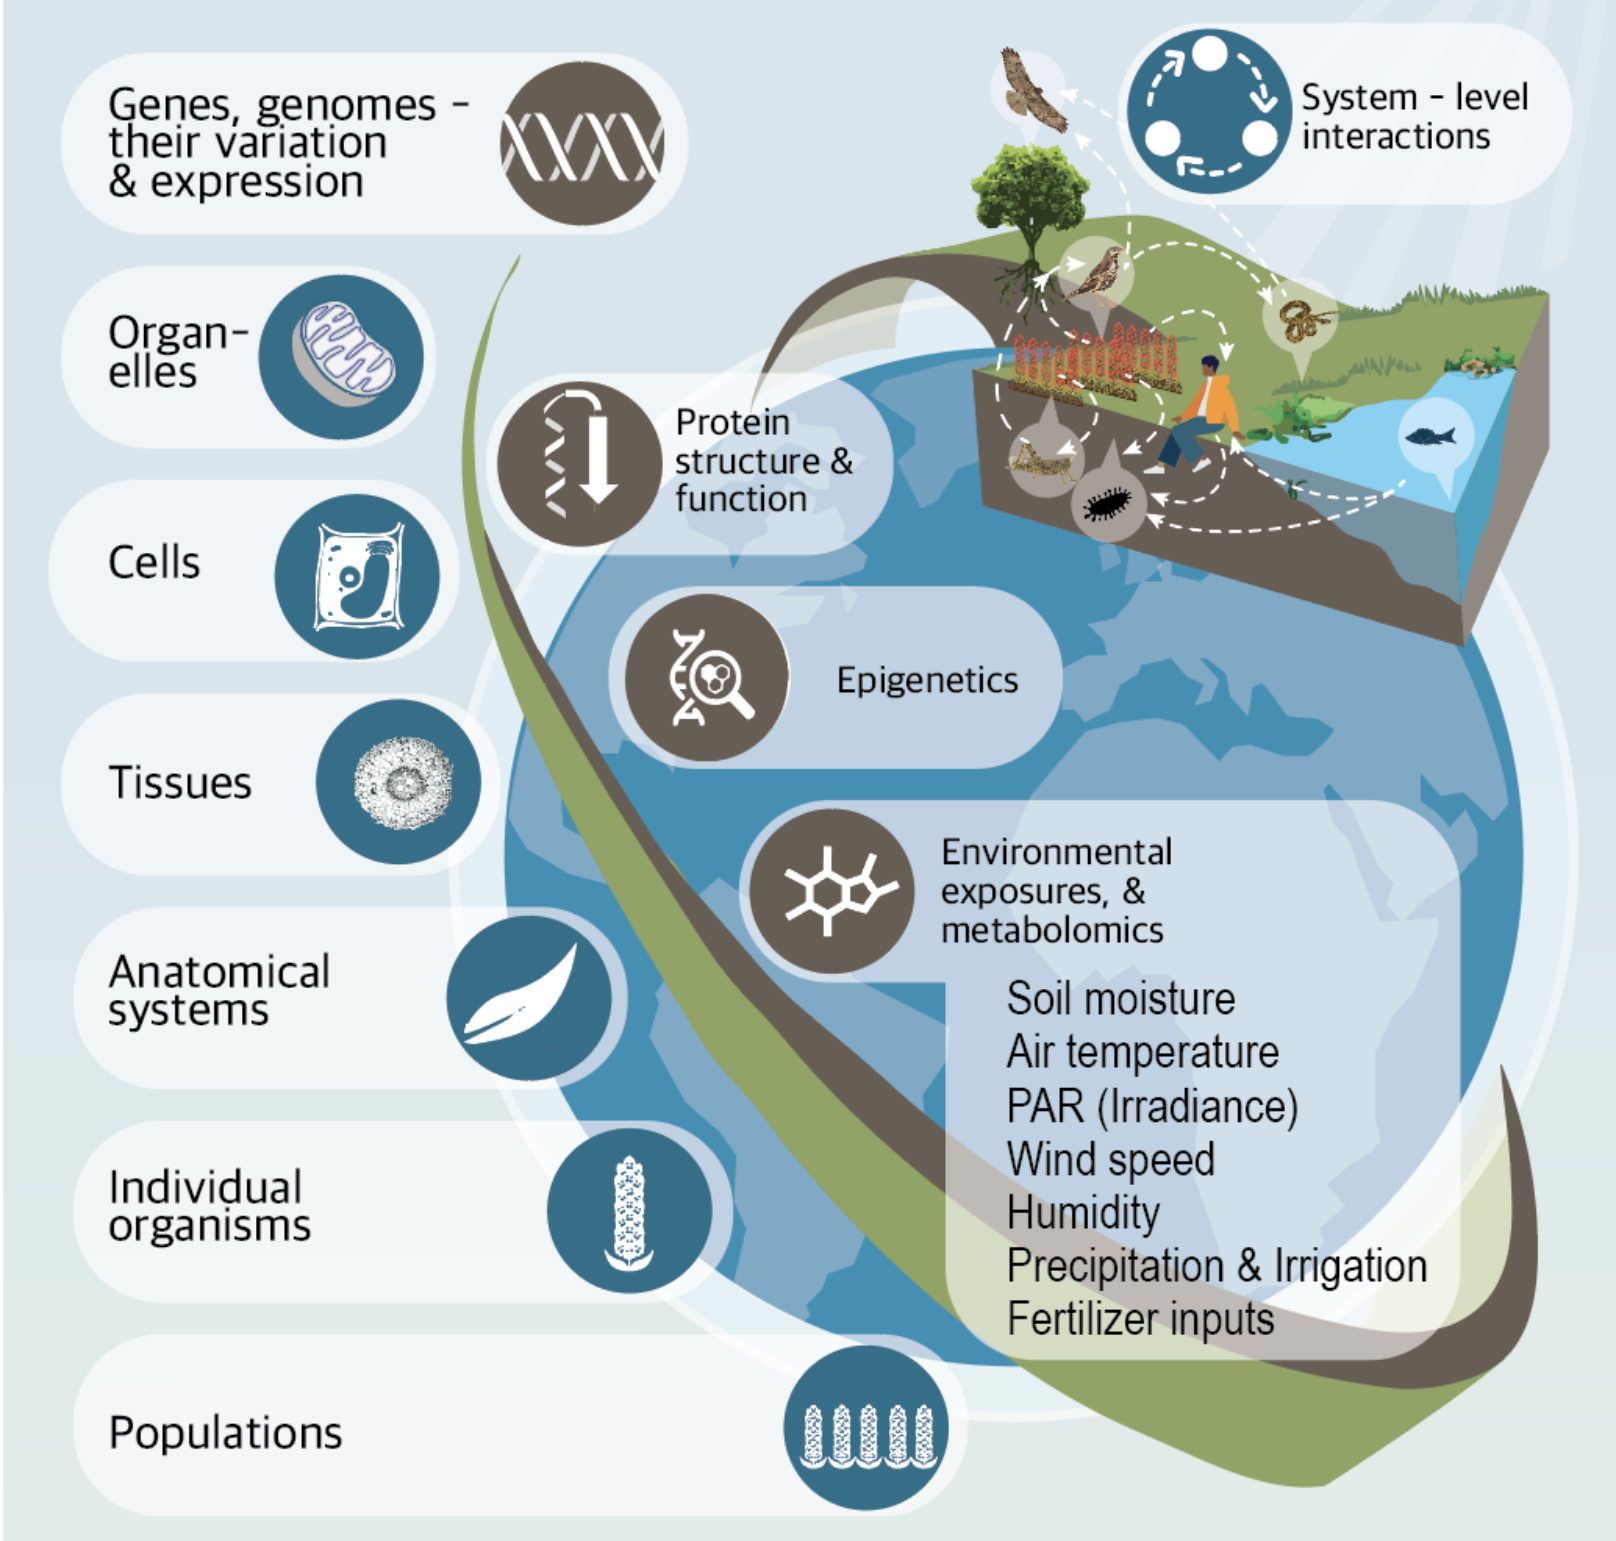
\includegraphics{Figure1.png}
\caption{System level interactions. Divided into environmental variation
(brown cartoons, right of line) interacting across all levels of
organismal structure (blue cartoons, left of line)}
\end{figure}

Existing models for predicting phenotypes from genetic and environmental
data focus on single species or single ecosystems. However, both
societal need and technical capabilities are moving toward addressing
larger scale questions that require integration of multi-modal data. In
addition to relatively small and heterogeneous data sets, researchers
are relying on national and global data collection efforts
\citep{balch2020neon} such as the National Ecological Observatory
Network (NEON) \citep{keller2008continental} and airborne and
space-based Earth Observation Systems (EOS). These efforts produce large
quantities of homogeneous ``born-digital'' data, but a significant
interdisciplinary data-integration task remains. Ontologies and
knowledge graphs using semantic similarity to cope with problems of
granularity and terminology (e.g.,
\citep{mungallintegrating2010, stuckyplant2018}) are now available to
facilitate data integration at scales beyond a single taxon or single
ecosystem. In addition, as the data sets and questions become more
complicated, more non-linear predictive models are needed to address
them.

\hypertarget{challenges-of-dataset-interoperability}{%
\section{Challenges of Dataset
Interoperability}\label{challenges-of-dataset-interoperability}}

Incorporating genomic data into phenomics is challenging. Many recent
studies have used only environmental features and machine learning to
predict phenotypes of lilacs, honeysuckle, rice, and wheat
\citep{ALDERMAN20171, nissanka2015calibration, mehdipoor2019geocomputational}.
There are a number of methods linking genomic data to environments or
traits. For example, genome wide association studies (GWAS) enable
researchers to examine the influence of single nucleotide polymorphisms
(SNP) on phenotypes in both natural and controlled settings
\citep{beyer2019loci, schlappi2017assessment, spindel2016genome}. GWAS
often provides generalized and mixed linear model associations between
SNPs and environmental variables, roughly analogous to Genes +
Environment = Phenotype (G+E=P). There are limitations in the
assumptions made by existing methodologies, such as GWAS, that directly
attribute plant phenotypes to environmental variables. These methods do
not explicitly incorporate biological and molecular interactions, such
as post-translational modification of macromolecules
\citep{running2014role}, the importance of plant-microbe interactions
\citep{oyserman2019extracting}, or endogenous siRNA
\citep{katiyar2006pathogen}. However, a machine learning approach allows
for these biological phenomena to be accounted for as latent variables
while probing the interactions of genomes, environments, and phenotypes
in a multidimensional manner.

Conventional observations and statistical models are shifting toward
remotely sensed observation and trait collection, which rely on machine
learning (ML) and computer vision for measurements. For example,
Bayesian Belief Networks \citep{cooper1990computational} may be
implemented to associate environmental variables with traits, and
Generative Adversarial Networks \citep{radford2015unsupervised} for
classifying plant phenotype imaging. Rather than simply generating large
quantities of machine readable data \citep{hampton2013big} and
implementing ML methods ad-hoc \citep{pichler2020machine}, ecologists
are now grappling with how to interpret the massive quantities of
unstructured data that are available at scale. Unfortunately, the ML
that provides a scalable, non-linear method for using these data, relies
on complex, ``black box'' methodologies to assess explanatory variables,
which does not aid interpretation. Here we introduce the GenoPhenoEnvo
project, an effort to predict phenotype from genetic and environmental
data, while developing novel representations of the ML ``black-box''
internals.

\hypertarget{future-directions}{%
\section{Future Directions}\label{future-directions}}

Our project has the long-term goal of developing predictive analytics
based on an organisms' genetic code and its associated phenotypic
response to environmental change. To design an initial analytical
framework and workflow, we will first use phenomic, genomic, and
environmental data about sorghum (\emph{Sorghum bicolor}). These data
are available through the TERRA-REF (Transportation Energy Resources
from Renewable Agriculture Phenotyping Reference Platform) project
\citep{lebauer2020data, burnette2018terra}. After training the ML model
on the highly controlled and thorough TERRA-REF data set, we aim to test
and further develop the model with data from less controlled and lower
resolution environments using data from sources such as NEON and the
National Phenology Network.

The first challenge is to prepare these data for use as input into ML
models. In addition to empirical data, ontologically-supported knowledge
graphs can be used to inform the ML \citep{mungall2017monarch}.
Knowledge graphs (KG) are directed acyclic graphs that represent
knowledge in a computational format and are an integral part of Google's
Answer Box and IBM's Watson. KGs can help constrain and prioritize
results, provide quality control, fill in data gaps with inferencing,
and integrate heterogeneous data. In this project, KGs provide an easier
way to integrate data from established plant phenome databases such as
Planteome \citep{cooper2018planteome}, Gramene
\citep{jaiswalgramene2011}, and TAIR \citep{pooletair2007}. The true
power of ontologies and KGs is a formal logical structure, enabling
inferential and similarity analyses
\citep{mungall2017monarch, washington2009linking}. In particular, it is
this latter feature that will enable data set interoperability. As we
begin to make predictions in more complicated systems with multiple
species and heterogeneous data, the knowledge graphs will be critical
for managing phenotype data.

The GenoPhenoEnvo (GPE) project aims to predict phenotype with genomic
and environmental data using a multimodal approach to training ML
models. We are actively developing a visualization tool to increase
understanding of why the model gave a particular result. In this way,
the GPE project will work toward phenotype predictions and an increased
understanding in the biological and molecular processes that translate
genotype to phenotype. In addition to increased awareness of molecular
effects, the ML models could enable specific ecological hypothesis
testing or predicting long-term speciation events driven by
environmental factors. Ultimately, we believe this combination of
methods will generate a new scientific sub-discipline, one we have
called ``\emph{Computational Ecogenomics.}''

\hypertarget{author-contributions}{%
\section{Author contributions}\label{author-contributions}}

The ordering of authors following RPB is alphabetical, contributions
included: conceptualization (c), editing (e), review (r), and text
writing (w).

RPB: cew AET: cerw AM: c; AR: c; DSL: cerw; EC: cr; ID: c; KS: c; MB: c;
MMT: cerw; PBH: c; PJ: c; RC: c; TLS: cerw.





\newpage
\singlespacing
\renewcommand\refname{References}
\bibliography{references.bib}

\end{document}
